\documentclass[10pt,twocolumn]{article}

\usepackage{times}
\usepackage{spverbatim}
\usepackage[utf8]{inputenc}
\usepackage{listings}
\usepackage[toc,page]{appendix}
\usepackage{graphicx}
\usepackage{mathtools}
\usepackage{float}
\renewcommand\appendixname{Bilagor}
\renewcommand\appendixpagename{Bilagor}

\raggedbottom
\sloppy

\title{Laborationsrapport i TSKS10 \emph{Signaler, Information och Kommunikation}}

\author{Martin Söderén \\ marso329, 9009291098 }

\date{\today}

\begin{document}

\maketitle

\section{Inledning}

Den här laborationen gick ut på analysera en delvis okänd signal. En del saker om den var givna men en del som krävdes för att kunna lyssna på signalen behövdes bestämma analytiskt. Signalen ser ut på följande sätt:

$$x(t)=x_I(t)\cos(2\pi f_c t)-x_Q(t)\sin(2\pi f_c t)+z(t)$$


\subsection{Givet}
\begin{itemize}
\item Bärfrekvensen $f_c$ är en multipel av 19 kHz
\item Signalen studsar mot ett objekt så ett eko uppstår. Tiden $\tau_1$ är tiden det tar från sändaren till mottagaren direkt. Tiden $\tau_2$ är tiden det tar från sändare till objekt och sedan till mottagare.
\item $\tau_2>\tau_1$ samt $\tau_2-\tau_1$ är en multipel av 1 ms. 
\item Första tredjedelen av $x_I(t)$ och $x_Q(t)$ innehåller varsin melodi.
\item Andra tredjedelen av $x_I(t)$ och $x_Q(t)$ innehåller varsitt ordspråk.
\item Sista tredjedelen av $x_I(t)$ och $x_Q(t)$ innehåller vitt brus.
\item Sändaren sänder samtidigt ut andra I/Q-modulerade signaler på andra bärfrekvenser. Dessa betecknas $z(t)$. 
\item Ekot gör att vi tar emot $y(t)=x(t-\tau_1)+0,9x(t-\tau_2)$
\item Signalen tas emot lågpassfiltrerad med ett idealt lågpassfilter
\item Samplingsfrekvensen är 400 kHz.
\end{itemize}

\section{Metod}

Uppgiften delades upp i tre mindre uppgifter: 
\begin{enumerate}
\item Ta reda på bärfrekvensen $f_c$
\item Ta reda på tidsfördröjningen $\tau_2-\tau_1$
\item I/Q modulera signalen
\end{enumerate}

\subsection{Bärfrekvens}
För att få fram bärfrekvensen så fouriertransformerades signalen och sedan plottades frekvensspektrumet. Detta kan ses i figur~\ref{fig:fft} under bilagor.
Här så ser man tre tydliga toppar. Dessa är vid 39200, 95000 och 133000 Hz.
\\
\\
Signalen filtreras för att få ut respektive signal med varsitt butterworthfilter. Signalerna plottas mot tiden och genom att mäta längden på datasignalen så ser man att det finns 7800000 sampel. Då samplingsfrekvensen var 400 kHz så är signalen 19.5 sekunder lång. Signalen med toppen vid 39200 Hz kan ses i 
figur~\ref{fig:first}, signalen med toppen vid 95000 Hz kan ses i figur~\ref{fig:second} och signalen med toppen vid 133000 Hz kan ses i figur~\ref{fig:third}.
\\
\\
Den första signalen ser ut att bara innehålla vitt brus. Den andra innehåller någonting periodiskt som troligtvis inte är intressant. Den tredje ser ut att innehålla användbar information så bärfrekvensen $f_c$ ansätts till 133 kHz.

\subsection{Tidsfördröjning}
För att få fram tidsfördröjning i signalen så autokorreleras det vita bruset som var den första signalen med toppen vid 39200 Hz. I figur~\ref{fig:tau} så kan man se en topp vid 19.5 s och två sidotoppar $\pm 0.41 $ s om toppen. Detta ger att $\tau_{2}-\tau_{1}=0.41$. Denna metod beskrivs och förklaras i kursboken kapitel 4.

\subsection{Filtrera bort eko}
Då tidsfördröjning och ekots amplitud nu är kända kan ekot filtreras bort. Detta görs genom att $x(t)=y(t)-0.9y(t-\tau) \text{ för alla } t>\tau$. I implementationen sker detta dock i block istället för varje enskilt sampel för att skynda på exekveringen. Efter filtreringen är bara den ursprungliga signalen kvar.

\subsection{I/Q-demodulering}
Signalen I/Q-demoduleras på följande sätt från kursboken avsnitt 1.4.2:
$$ x_I(t)= \mathcal{H}^{LP}_{B/2}\{ 2x(t)\cos(2 \pi f_c t) \}$$
$$ x_Q(t)= -\mathcal{H}^{LP}_{B/2}\{ 2x(t)\sin(2 \pi f_c t) \}$$
Där $B$ är signalens bandbredd men det är känt att signalen bara ska innehålla tal så signalen lågpassfiltreras med gränsfrekvensen 20 kHz istället. Bärfrekvensen $f_c$ är känd från avsnitt 2.1 och är 133 kHz.
\\
\\
Detta ger två signaler som spelas upp efter nedsampling. Matlab kunde inte spela upp ljud i 400 kHz så signalerna nedsamplades till 100 kHz. 

\section{Resultat}

Den sökta informationen är:
\begin{itemize}
\item Bärfrekvensen $f_c$ är 133 kHz
\item Tidsfördröjningen $\tau_2-\tau_1$ är 410 ms.
\item Ena delen innehöll först ett pianostycke, sedan ordspråket "Den som ger sig in i leken får leken tåla" och sedan vitt brus
\item Andra delen innehöll först ett pianostycke, sedan ordspråket "Även små grytor har öron" och sedan vitt brus.

\subsection{Anmärkning}
Om det uppkommer en fasförskjutning på $\frac{\pi}{2}$ så kan $x_I(t)$ och $x_Q(t)$ byta plats. Så man kan inte vara säker på att signalen som demodulerades till $x_I(t)$ var signalen som modulerades och sändes som $x_I(t)$.
\end{itemize}


\begin{figure}[H]
	\begin{center}
		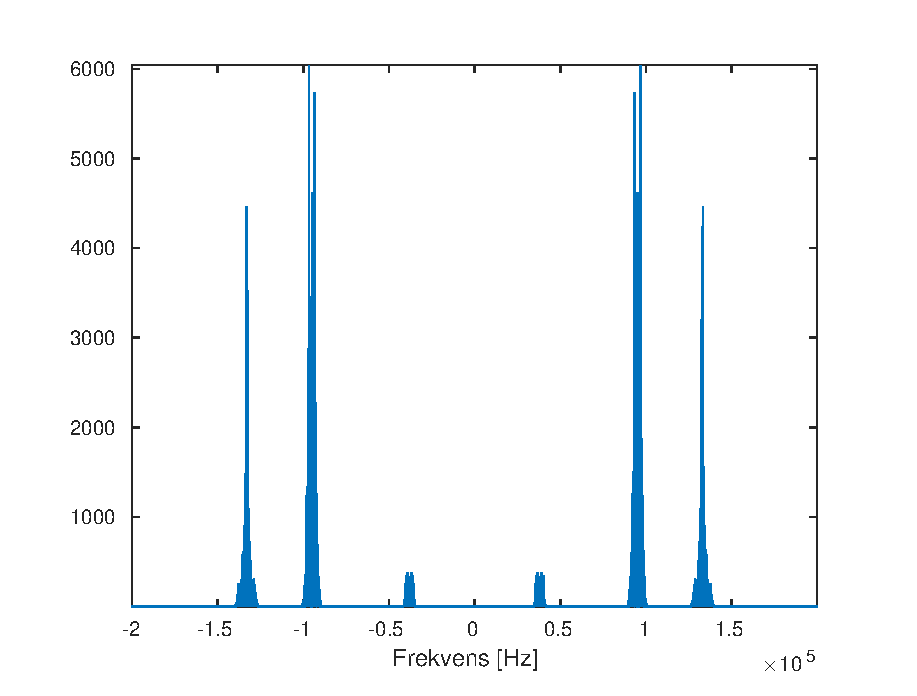
\includegraphics[scale=0.5]{fft.eps}
	\end{center}
	\caption{Fouriertranform av signalen.}
	\label{fig:fft}
\end{figure}

\begin{figure}[H]
	\begin{center}
		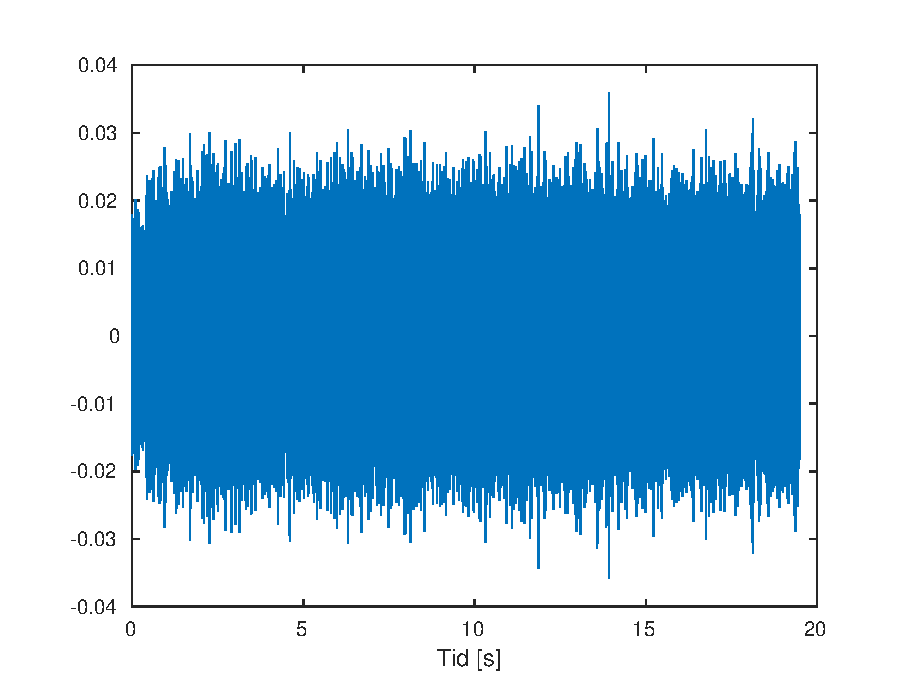
\includegraphics[scale=0.5]{first.eps}
	\end{center}
	\caption{Första signalen.}
	\label{fig:first}
\end{figure}

\begin{figure}[H]
	\begin{center}
		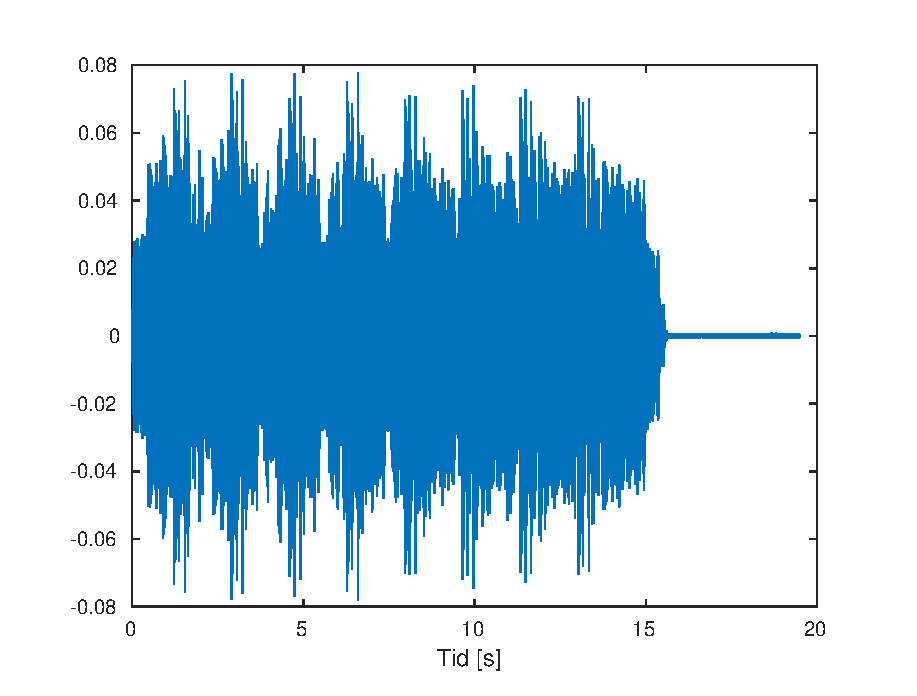
\includegraphics[scale=0.5]{second.eps}
	\end{center}
	\caption{Andra signalen.}
	\label{fig:second}
\end{figure}

\begin{figure}[H]
	\begin{center}
		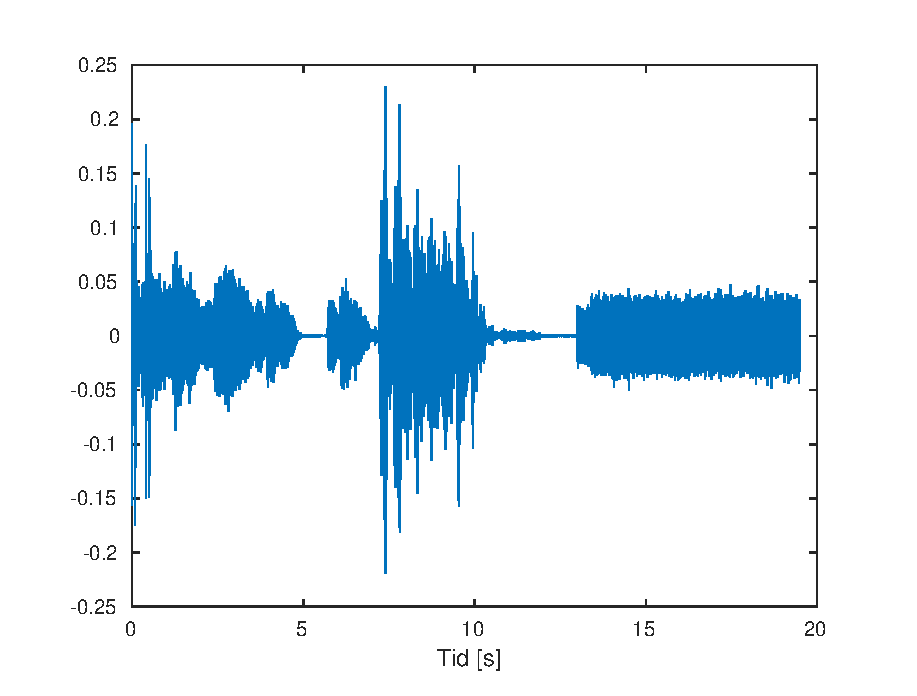
\includegraphics[scale=0.5]{third.eps}
	\end{center}
	\caption{Tredje signalen.}
	\label{fig:third}
\end{figure}

\begin{figure}[H]
	\begin{center}
		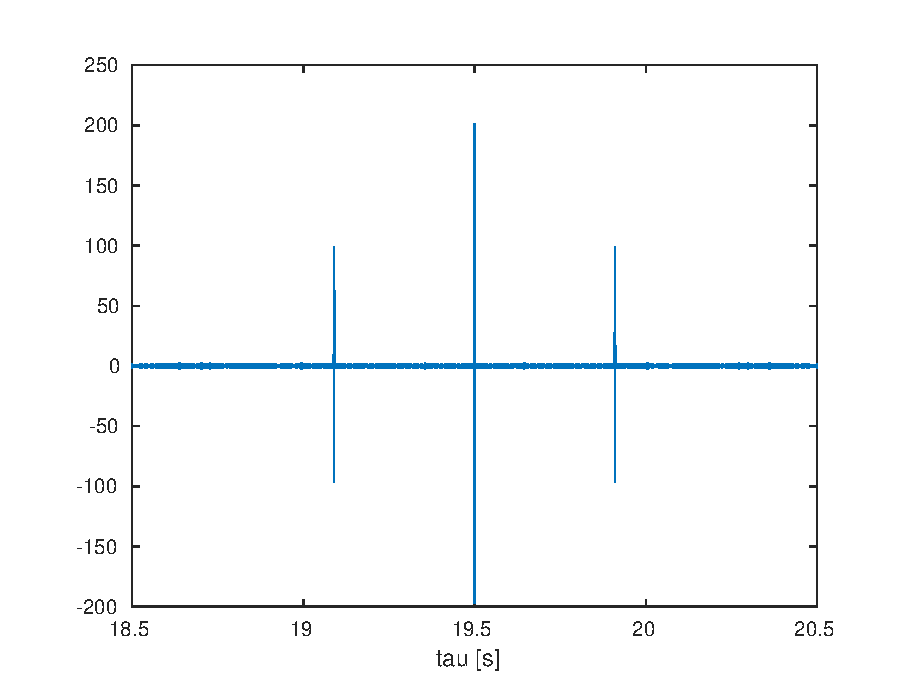
\includegraphics[scale=0.5]{tau.eps}
	\end{center}
	\caption{Autokorrelationen av det vita bruset}
	\label{fig:tau}
\end{figure}

\newpage
\onecolumn
\section*{Min Matlab-kod:}
\lstinputlisting[language=matlab]{tsks10.m}
\end{document}
